\documentclass[twocolumn]{article}
\usepackage{sample}
\usepackage{verbatim}
\usepackage{graphicx}
\usepackage{tabularx}
\usepackage[htt]{hyphenat}

\newcommand{\naive}{Na\"\i ve}
\newcommand{\method}[1]{\texttt{#1()}}
\newcommand{\class}[1]{\texttt{#1}}
\newcommand{\param}[1]{\texttt{#1}}
\newcommand{\aicat}{\texttt{AI::Cat\-e\-gor\-i\-zer}}


\raggedbottom
\def\BibTeX{{\rm B\kern-.05em{\sc i\kern-.025em b}\kern-.08em
    T\kern-.1667em\lower.7ex\hbox{E}\kern-.125emX}}

\title{Automatic Categorization of Announcements \\ on the Australian Stock Exchange}

\author{
{\em Rafael A. Calvo}\\[1ex]
Web Engineering Group\\
The University of Sydney\\
Bldg J03, Sydney NSW 2006\\[1ex]
{\em rafa@ee.usyd.edu.au}
\and
{\em Ken Williams}\\[1ex]
Web Engineering Group\\
The University of Sydney\\
Bldg J03, Sydney NSW 2006\\[1ex]
{\em kenw@ee.usyd.edu.au}
}
\date{}

\begin{document}

\maketitle
\thispagestyle{empty}

        \begin{figure}[b]
	~\\
        \noindent
        {\small\bf\raggedright
        Proceedings of the 7th Australasian 
	Document Computing Symposium,\\
	Sydney, Australia,
        December 16, 2002.
        }
        \end{figure}


\subsection*{\centering Abstract}
%IEEE allows italicized abstract
\noindent
{\it 
This paper compares the performance of several machine learning
algorithms for the automatic categorization of corporate announcements
in the Australian Stock Exchange (ASX) Signal G data stream. The
article also describes some of the applications that the
categorization of corporate announcements may enable. We have
performed tests on two categorization tasks: market sensitivity, which
indicates whether an announcement will have an impact on the market,
and report type, which classifies each announcement into one of the
report categories defined by the ASX. We have tried Neural Networks, a
\naive\ Bayes classifier, and Support Vector Machines and achieved
good results.
}

\paragraph{Keywords} 
Document Management, Document Workflow

\section{Introduction}
\label{introduction}

The Australian Stock Exchange Limited (ASX - http://www.asx.com.au/)
operates Australia's primary national stock exchange.  Companies
listed on ASX are required under the Listing Rules to make
announcements about their activities "in order to ensure a fully
informed market is maintained." \cite{asx:02} In order to guarantee
access to this information, stock exchanges such as the ASX publish
all recent and historical company announcements.  Thanks to language
technologies such as automatic document categorization, these
corporate announcements can provide new sources of valuable financial
information.

Historically, corporate announcements have provided valuable
information to traders and the general public for decades. For this
reason these announcements are used by regulators as the main tool to
keep the market informed of all important events. The law assumes that
these public announcements contain all the information needed by an
individual trader to keep a reasonable understanding of what is
happening with a particular company. This allows investors to make
decisions based on information that is up to date and is equivalent to
the information that company insiders might have. There is little
doubt about the value of the information contained in these
announcements, and several research groups are developing
novel applications using this data.  We describe in this article
the evaluation of categorization techniques used to build these
applications.

The ASX Data Services is a financial information service providing
daily market information from the Stock Exchange Automated Trading
System (SEATS), ASX futures and the company announcement service.  All
daily stock exchange activity is available in different electronic
data feeds that the ASX calls ``signals.''  In our work, we have used
announcements from the ASX's Signal G, which provides subscribers with
company announcements issued by companies or the ASX in accordance
with listing rules.

Section \ref{data} of this paper
describes the Signal G data set.  Section \ref{methods} describes the
different machine learning techniques and the categorization framework
that we have used to perform these types of categorization
tasks. Section \ref{results} describes the quantitative results and
section \ref{conclusion} concludes.

\section{Data Description}
\label{data}

In this paper we assess performance on two tasks: ``report type'' and
``market sensitivity'' categorization. Report type is ``a code to
categorize company announcements'' \cite{asx:02} and may take one of 144 values
like ``annual report'' or ``takeover announcement.'' Market
sensitivity is a boolean category indicating whether an announcement
contains information that may influence trading in the issuing
company. This allows users of this data to select which announcements
are critical.

Currently, both kinds of category assignments on the Signal G
documents are made manually by the ASX.  Table
\ref{signalg-sensitivity} shows the distribution of documents with
respect to the sensitivity category, as well as our split between
training and testing documents.  Figure \ref{signalg-reptype} shows
the report type category distribution.


\begin{table}
\begin{tabular}{|r|r|r|r|}
\hline
         & Sensitive & Nonsensitive & Total \\
\hline
Training & 32458     & 63067        & 95525 \\
\hline
Test     & 14072     & 27033        & 41405 \\
\hline
Total    & 46530     & 90100        & 136630\\
\hline
\end{tabular}
\caption{Sensitivity category distribution in Signal G}
\label{signalg-sensitivity}
\end{table}

Note that the report type labels are highly skewed across categories.  The most
common category contains 10,064 documents, while ten categories have
fewer than five documents each.

\begin{figure}
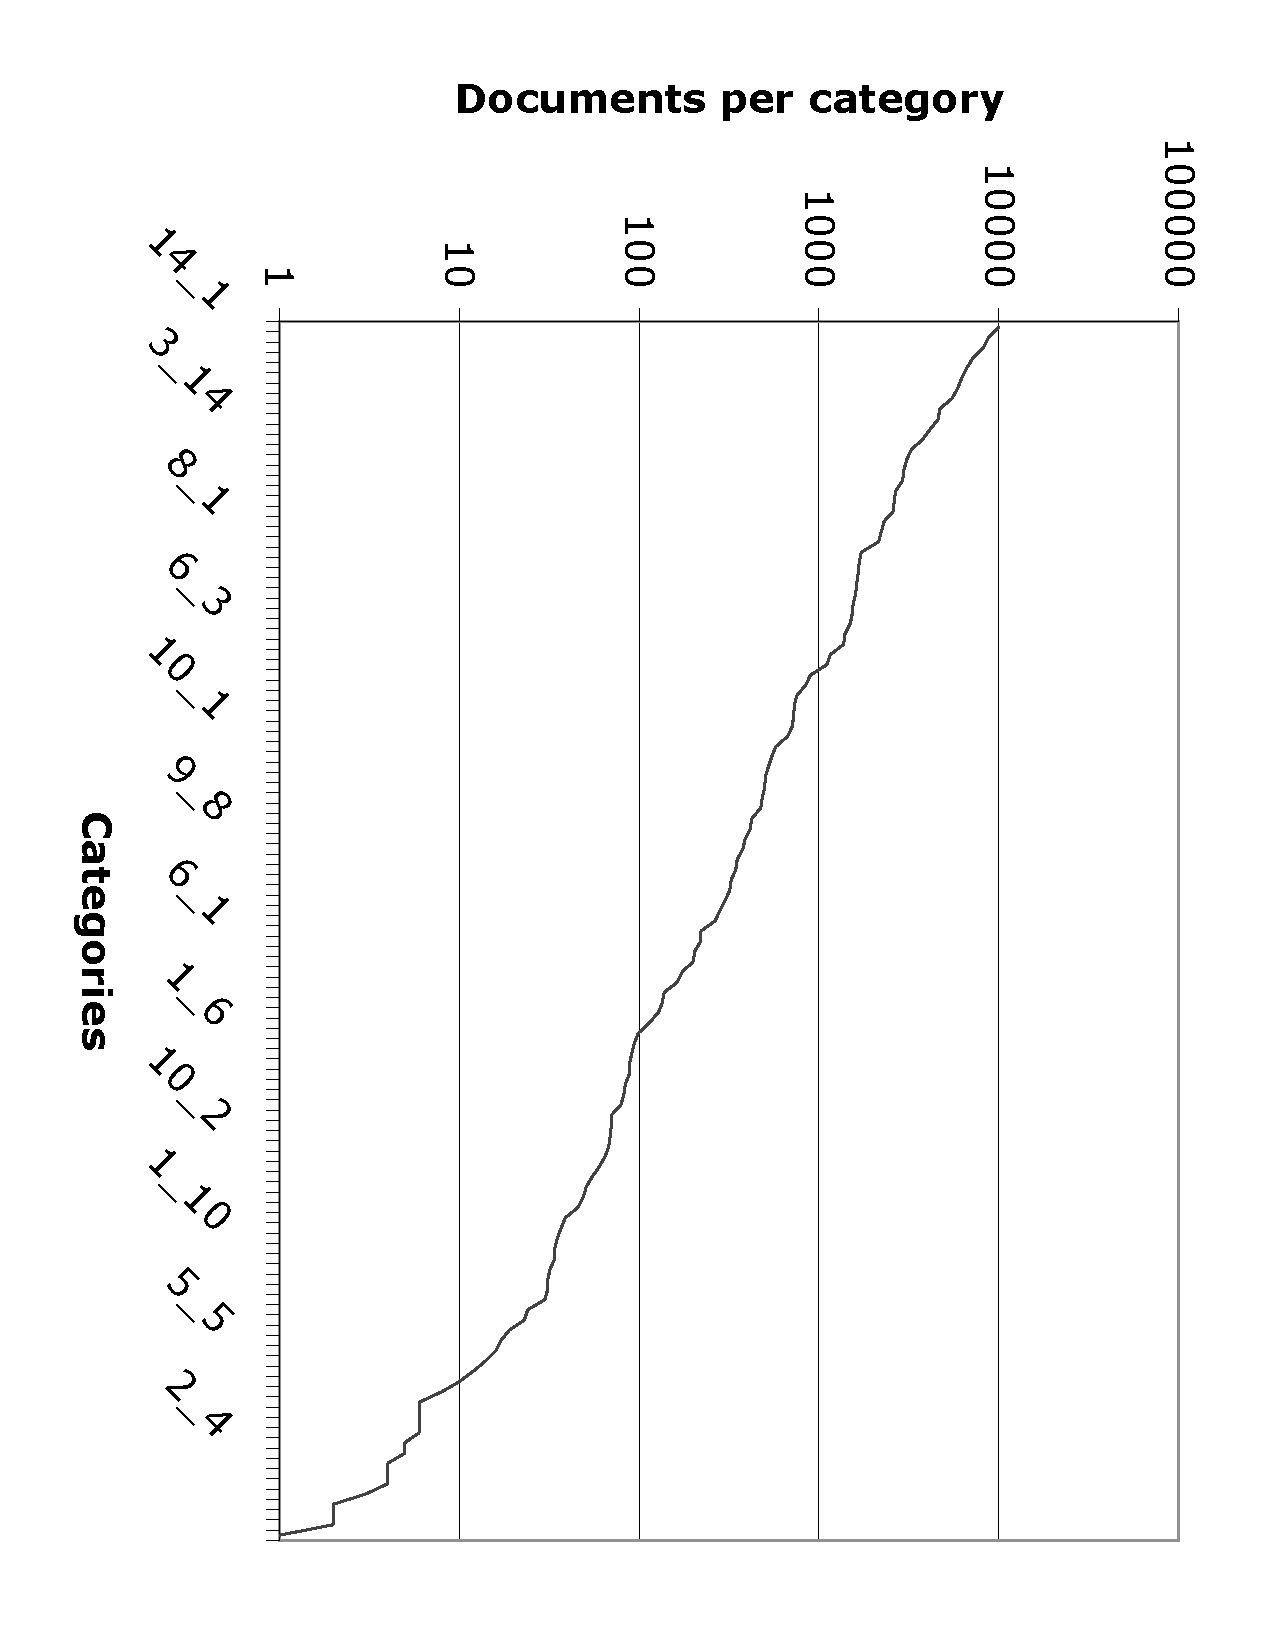
\includegraphics[angle=90,width=\linewidth]{signalg-reptype}
\caption{Report type category distribution in Signal G}
\label{signalg-reptype}
\end{figure}

Signal G is available to the public, member organizations, and
information vendors.  Our data set was supplied by the Capital Markets
Collaborative Research Centre.  For future groups who receive
permission from the CMCRC to work with this data, we have converted it
into an XML format.



\section{Methods}
\label{methods}


We have compared three machine learning methods that have provided
some of the best performances in other classification tasks
\cite{yang:99}: Support Vector Machines (SVM) \cite{scholkopf:99}
\cite{joachims:99}, \naive\ Bayes (NB) \cite{lewis:98}, and Neural
Networks (NN) \cite{calvo:00} \cite{calvo:01}. It is not possible to
describe them thoroughly in this article, so we will only summarize
those issues that might be required to reproduce the results.  Our
\naive\ Bayes and SVM implementations are described in
\cite{williams:02}.

Because of the inability of our SVM implementation to handle the size
of our training set, we had to only train on 8000 documents at a time
in order to finish the experiments in a reasonable amount of time.
The SVM was not able to perform the report type task, only the sensitivity
task.  Future work may dramatically improve training speed by using
recently developed training optimizations in the literature, enabling
us to train on a larger number of documents and presumably to improve
our correctness as a result.

Our Neural Network architecture \cite{calvo:00} \cite{calvo:01} used a
backpropagation algorithm that minimizes quadratic error. The input
layer has as many units (neurons) as document features retained. The
number of hidden units is determined by optimising the performance on
a cross-validation set. There is one output unit for each possible
category, with activation values between 0 and 1. For each document,
the classifier will assign any category whose output unit is greater
than 0.5. In our experiment, we used 3-fold cross-validation and
averaged the weights of the three resultant neural networks.

Each categorizer was trained on the 95,525 training documents for each
task, report type and sensitivity.  For the Neural Network
categorizer, 13,711 training documents were set aside from the
training set to function as a validation set when tuning the weights
of the network.  The trained categorizers were then evaluated on the
41,405 test documents. Since documents in the test set have not been
used to adjust the parameters of the classifier, it is normally
assumed that the performance on new data would be similar.

Table \ref{algos} summarizes the general steps followed in the
preparation of the experiments.  TF/IDF weights are given in the
notation followed by \cite{salton:88}.  Our experimental process was
as follows:

\begin{enumerate}

\item Linguistic dimensionality reduction: A list of stopwords
\cite{salton:89} was removed from the document collection and the
Porter stemming algorithm was applied \cite{manning:99}.
\item Statistical dimensionality reduction: Chi Squared or Document
Frequency criteria were employed to reduce the feature
vector dimensionality \cite{manning:99} \cite{sebastiani:02}.
\item Vectorization and weighting: The resulting documents were
represented as vectors, using TF/IDF weighting \cite{salton:88}
\cite{yang:97}.
\item Architecture: The selected terms were used as input features to
the classifier. Some of the algorithms allow several architectures,
and the best algorithm was chosen by optimising the results on a
cross-validation set.
\item Training: We generated a cross-validation set randomly. These
documents were set aside and the Neural Network was trained on the
remaining ones.


\end{enumerate}

\begin{table*}
\begin{tabularx}{\linewidth}{|r|l|l|l|l|X|}
\hline
& Stopwords & Stemming & Feature Reduction & TF/IDF & Architecture\\
\hline
NN & SMART & Porter & $\chi^2$ & tfc & 1000 features, 50 hidden units \\
\hline
NB & SMART & Porter & DF & tfx & 1000 features \\
\hline
SVM & SMART & Porter & DF & tfx & 1000 features, linear kernel \\

\hline
\end{tabularx}
\caption{Comparative description of algorithms used}
\label{algos}
\end{table*}


\section{Results}
\label{results}

In evaluating our classifiers on our data set, we use the common
statistical measures \emph{precision}, \emph{recall}, and
$F_1$. \cite{yang:99} \cite{rijsbergen:79} When dealing with multiple
classes there are two possible ways of averaging these measures,
\emph{macro-averaging} and \emph{micro-averaging}. The macro-average
weights equally all the classes, regardless of how many documents they
contain. The micro-average weights equally all the documents, thus
biasing toward the performance on common classes.  Since different
learning algorithms will perform differently on common and rare
categories, both micro-averaged and macro-averaged scores are
typically reported to evaluate performance.

\begin{table}
\begin{tabular}{|c|c|c|c|c|c|c|}
\hline
   & \multicolumn{3}{|c|}{Micro} & \multicolumn{3}{|c|}{Macro} \\
\hline
   & $p$  & $r$  &$F_1$ & $p$  & $r$  & $F_1$ \\
\hline
 NN & 0.89 & 0.89 & 0.89 & 0.88 & 0.88 & 0.88 \\
 NB & 0.83 & 0.84 & 0.83 & 0.90 & 0.90 & 0.90 \\
SVM & 0.82 & 0.82 & 0.82 & 0.80 & 0.79 & 0.80 \\
\hline
\end{tabular}
\caption{Performance for the market sensitivity task}
\label{res:sens}
\end{table}


\begin{table}
\begin{tabular}{|c|c|c|c|c|c|c|}
\hline
   & \multicolumn{3}{|c|}{Micro} & \multicolumn{3}{|c|}{Macro} \\
\hline
   & $p$  & $r$  &$F_1$ & $p$  & $r$  & $F_1$ \\
\hline
NN & 0.87 & 0.71 & 0.78 & 0.45 & 0.34 & 0.37  \\
NB & 0.62 & 0.67 & 0.64 & 0.46 & 0.61 & 0.46  \\
\hline
\end{tabular}
\caption{Performance for the report type task}
\label{res:rept}
\end{table}

It is important to note that the performance results are based on
comparing the automatic categorization of each document with the
tagging of human experts at the ASX. The manual classification is a
subjective decision process affected by the ASX's legal liabilities
and the normal human classification disagreements. It has been shown
in various studies that there could be considerable variation in the
inter-indexer agreement \cite{bruce:98} \cite{brants:00}. For example,
in a Reuters news collection correction rates averaged 5.16\%
\cite{rose:02} with some editors being corrected up to 77\% of the
time. Similar disagreements can be expected in the ASX's assignments
on the Signal G corpus.  In the light of these disagreements we can
imagine that there might be a limit to the performance that can be
obtained by automatic categorization.

Figure \ref{histogram} shows a histogram of classes and documents for
different performance ranges using the \naive\ Bayes classifier. It
shows how most categories that do well have large number of documents,
except for some that have very few documents (fewer than 5). This
shows the well-known result that the machine learning algorithms such
as \naive\ Bayes perform better on well-populated
categories. Similar results can be obtained for the other classifiers.


\begin{figure}
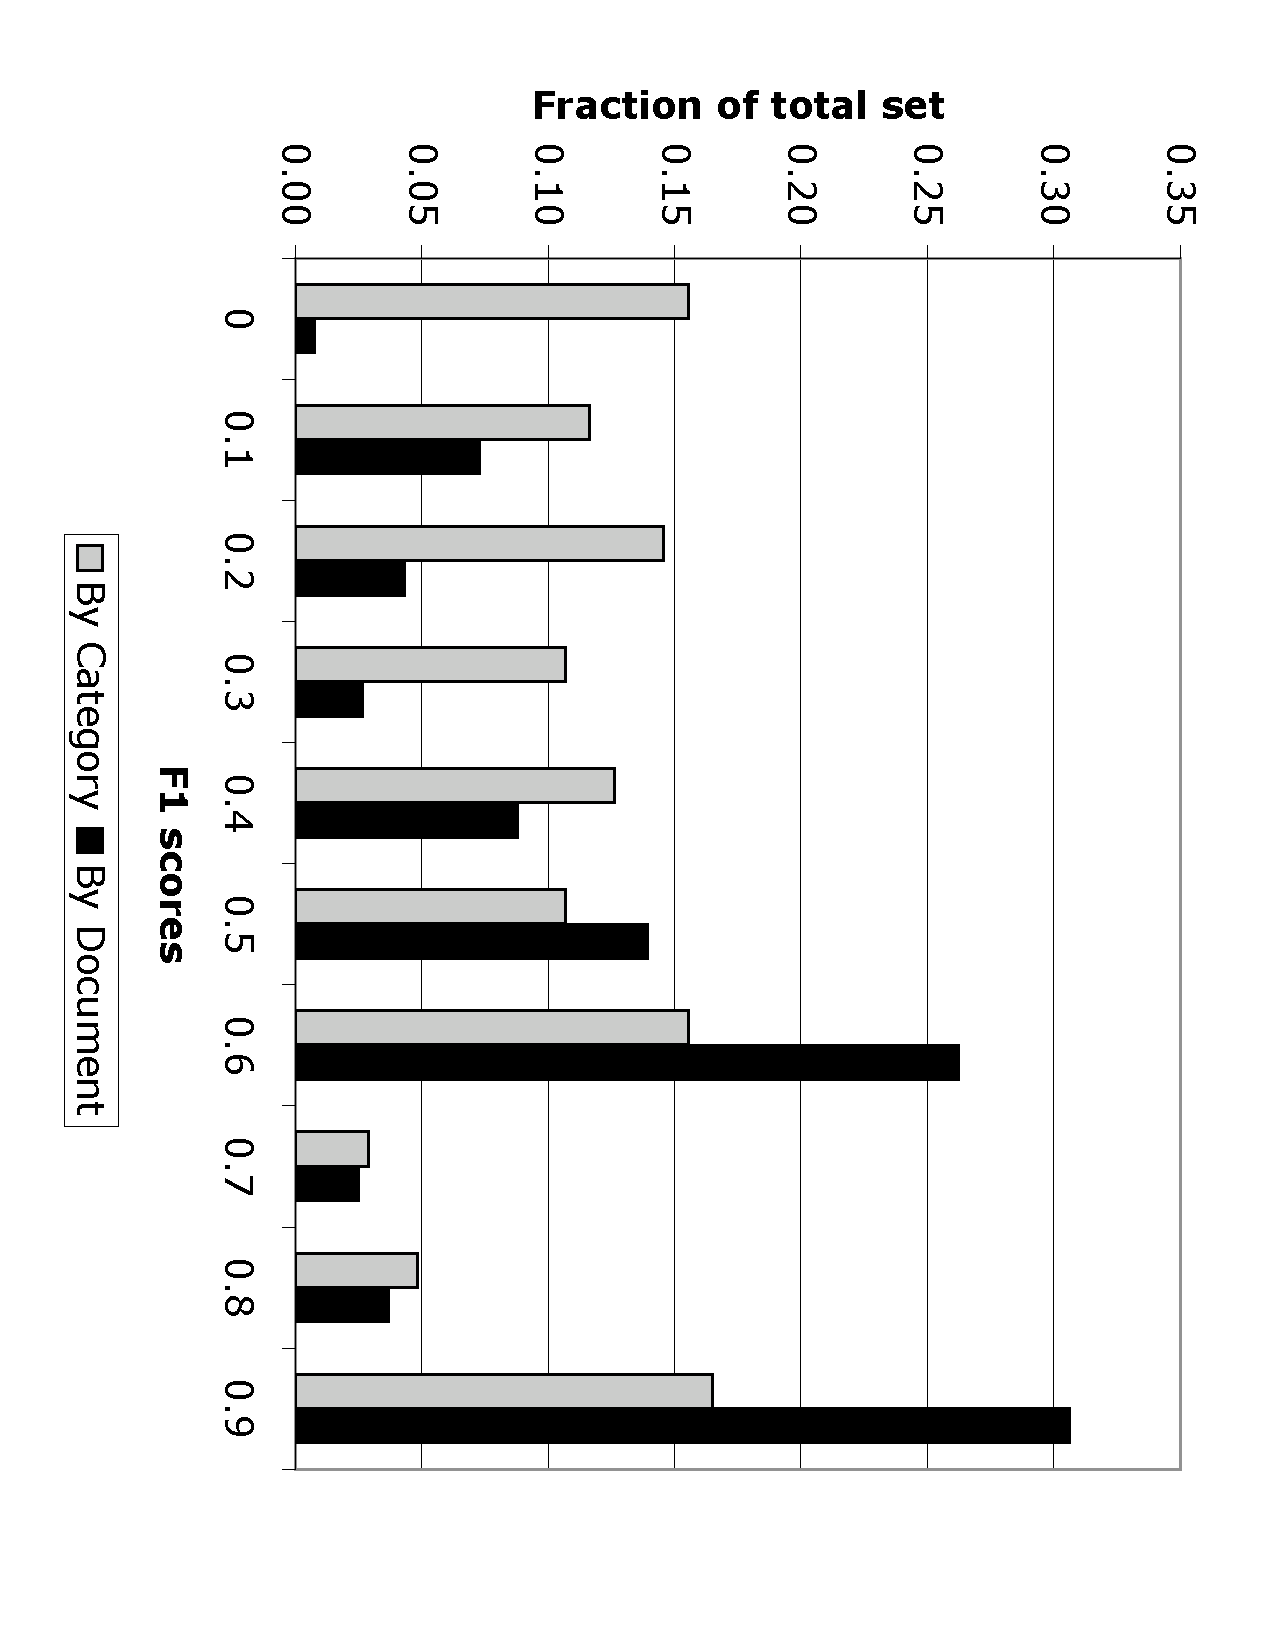
\includegraphics[angle=90,width=\linewidth]{results}
\caption{Histogram of report type results for different performance ranges}
\label{histogram}
\end{figure}

\section{Conclusion}
\label{conclusion}


In this paper we have applied several machine learning techniques
(Neural Networks, \naive\ Bayes, and Support Vector Machines) to the
categorization of announcements of companies publicly traded by the
ASX.  Two tasks were evaluated: the categorization of documents as
sensitive or not, and the categorization in one of the 144 report
types defined by ASX. The results show that is possible to obtain
classifiers with more than 88\% precision and recall on the
sensitivity task and 86\% precision, 74\% recall on the report type
task.

The results are somewhat better than the ones obtained by several
researchers working on the Reuters news cable database \cite{calvo:00}
\cite{calvo:01}. This database has fewer categories (90) than the
report type task but also fewer documents (10,000). Although it is
risky to try to extrapolate the results, we believe that due to the
similarity in the documents, other financial databases with documents
in English should also have similar performance. Future work includes
testing adding statistical feature selection to the classification
framework, and improving the efficiency of the algorithms so they can
be used for even larger data sets.

The excellent performance shows the possibility to use these
classifiers in commercial applications for both tasks, sensitivity
detection and report type categorization.


\section*{Acknowledgements}

The authors gratefully acknowledge financial support from the Capital
Markets Collaborative Research Centre and the University of Sydney.


\bibliographystyle{sample}
\bibliography{TC-references}

\end{document}
